
%\subsection{Discussion}
%\label{sec:dsc}

%Let us look at both our techniques in the context of Zenger and Odersky 
%challenge to independently extensible solutions of extension problem discussed 
%in \textsection\ref{sec:exp}.

%\begin{itemize}
%\item Extensibility in both dimensions: \\
%      %It should be possible to add new data variants, while adapting the 
%      %existing operations accordingly. It should also be possible to introduce 
%      %new functions. 
%      Our techniques allow one to extend data with subclassing as well as 
%      introduce new functions through a match statement on corresponding 
%      encoding. The existing operations 
%\item Strong static type safety: \\
%      %It should be impossible to apply a function to a data variant, which it 
%      %cannot handle.
%\item No modification or duplication: \\
%      %Existing code should neither be modified nor duplicated.
%\item Separate compilation: \\
%      %Neither datatype extensions nor addition of new functions should require 
%      %re-typechecking the original datatype or existing functions. No safety 
%      %checks should be deferred until link or runtime.
%\item Independent extensibility: \\
%      %It should be possible to combine independently developed extensions so 
%      %that they can be used jointly.
%\end{itemize}
%
\section{Evaluation} %%%%%%%%%%%%%%%%%%%%%%%%%%%%%%%%%%%%%%%%%%%%%%%%%%%%%%%%%%%
\label{sec:eval}

\begin{figure*}
\begin{tabular}{@{}c@{ }l||@{ }r@{}@{ }r@{}@{ }r@{}|@{ }r@{}@{ }r@{}@{ }r@{}||@{ }r@{}@{ }r@{}@{ }r@{}|@{ }r@{}@{ }r@{}@{ }r@{}||@{ }r@{}@{ }r@{}@{ }r@{}|@{ }r@{}@{ }r@{}@{ }r@{}}
\hline % -----------------------------------------------------------------------------------------------------------------------------------------
\hline % -----------------------------------------------------------------------------------------------------------------------------------------
 &            & \multicolumn{6}{c||}{G++/32 on Windows Laptop} & \multicolumn{6}{c||}{MS Visual C++/32}        & \multicolumn{6}{c}{MS Visual C++/64}           \\
\hline % -----------------------------------------------------------------------------------------------------------------------------------------
 & Syntax     & \multicolumn{3}{c|}{Unified} & \multicolumn{3}{c||}{Specialized} & \multicolumn{3}{c|}{Unified} & \multicolumn{3}{c||}{Specialized} & \multicolumn{3}{c|}{Unified} & \multicolumn{3}{c}{Specialized} \\
\hline % -----------------------------------------------------------------------------------------------------------------------------------------
 & Encoding   & \Opn  & \Cls  & \Unn  & \Opn  & \Cls  & \Unn  & \Opn  & \Cls  & \Unn  & \Opn  & \Cls  & \Unn  & \Opn  & \Cls  & \Unn  & \Opn  & \Cls  & \Unn   \\
\hline % -----------------------------------------------------------------------------------------------------------------------------------------
\hline % -----------------------------------------------------------------------------------------------------------------------------------------
 & Repetitive &\gwNGPp&\gwNGKp&\gwNGUp&\gwNSPp&\gwNSKp&\gwNSUp&\vwNGPp&\vwNGKp&\vwNGUp&\vwNSPp&\vwNSKp&\vwNSUp&\vxNGPp&\vxNGKp&\vxNGUp&\vxNSPp&\vxNSKp&\vxNSUp \\
 & Sequential &\gwNGPq&\gwNGKq&\gwNGUq&\gwNSPq&\gwNSKq&\gwNSUq&\vwNGPq&\vwNGKq&\vwNGUq&\vwNSPq&\vwNSKq&\vwNSUq&\vxNGPq&\vxNGKq&\vxNGUq&\vxNSPq&\vxNSKq&\vxNSUq \\
 & Random     &\gwNGPn&\gwNGKn&\gwNGUn&\gwNSPn&\gwNSKn&\gwNSUn&\vwNGPn&\vwNGKn&\vwNGUn&\vwNSPn&\vwNSKn&\vwNSUn&\vxNGPn&\vxNGKn&\vxNGUn&\vxNSPn&\vxNSKn&\vxNSUn \\
\hline % ------------------------------------------------------------------------------------------------------------------------------------------
\multirow{3}{*}{\begin{sideways}{\tiny Forward}\end{sideways}}
 & Repetitive &\gwYGPp&\gwYGKp&\gwYGUp&\gwYSPp&\gwYSKp&\gwYSUp&\vwYGPp&\vwYGKp&\vwYGUp&\vwYSPp&\vwYSKp&\vwYSUp&\vxYGPp&\vxYGKp&\vxYGUp&\vxYSPp&\vxYSKp&\vxYSUp \\
 & Sequential &\gwYGPq&\gwYGKq&\gwYGUq&\gwYSPq&\gwYSKq&\gwYSUq&\vwYGPq&\vwYGKq&\vwYGUq&\vwYSPq&\vwYSKq&\vwYSUq&\vxYGPq&\vxYGKq&\vxYGUq&\vxYSPq&\vxYSKq&\vxYSUq \\
 & Random     &\gwYGPn&\gwYGKn&\gwYGUn&\gwYSPn&\gwYSKn&\gwYSUn&\vwYGPn&\vwYGKn&\vwYGUn&\vwYSPn&\vwYSKn&\vwYSUn&\vxYGPn&\vxYGKn&\vxYGUn&\vxYSPn&\vxYSKn&\vxYSUn \\
\hline % -----------------------------------------------------------------------------------------------------------------------------------------
\hline % -----------------------------------------------------------------------------------------------------------------------------------------
 &            & \multicolumn{6}{c||}{G++/32 on Linux Desktop} & \multicolumn{6}{c||}{MS Visual C++/32 with PGO} & \multicolumn{6}{c}{MS Visual C++/64 with PGO} \\
\hline % -----------------------------------------------------------------------------------------------------------------------------------------
 & Syntax     & \multicolumn{3}{c|}{Unified} & \multicolumn{3}{c||}{Specialized} & \multicolumn{3}{c|}{Unified} & \multicolumn{3}{c||}{Specialized} & \multicolumn{3}{c|}{Unified} & \multicolumn{3}{c}{Specialized} \\
\hline % -----------------------------------------------------------------------------------------------------------------------------------------
 & Encoding   & \Opn  & \Cls  & \Unn  & \Opn  & \Cls  & \Unn  & \Opn  & \Cls  & \Unn  & \Opn  & \Cls  & \Unn  & \Opn  & \Cls  & \Unn  & \Opn  & \Cls  & \Unn   \\
\hline % -----------------------------------------------------------------------------------------------------------------------------------------
\hline % -----------------------------------------------------------------------------------------------------------------------------------------
 & Repetitive &\glNGPp&\glNGKp&\GwNGUp&\glNSPp&\glNSKp&\GwNSUp&\VwNGPp&\VwNGKp&\VwNGUp&\VwNSPp&\VwNSKp&\VwNSUp&\VxNGPp&\VxNGKp&\VxNGUp&\VxNSPp&\VxNSKp&\VxNSUp \\
 & Sequential &\glNGPq&\glNGKq&\GwNGUq&\glNSPq&\glNSKq&\GwNSUq&\VwNGPq&\VwNGKq&\VwNGUq&\VwNSPq&\VwNSKq&\VwNSUq&\VxNGPq&\VxNGKq&\VxNGUq&\VxNSPq&\VxNSKq&\VxNSUq \\
 & Random     &\glNGPn&\glNGKn&\GwNGUn&\glNSPn&\glNSKn&\GwNSUn&\VwNGPn&\VwNGKn&\VwNGUn&\VwNSPn&\VwNSKn&\VwNSUn&\VxNGPn&\VxNGKn&\VxNGUn&\VxNSPn&\VxNSKn&\VxNSUn \\
\hline % ------------------------------------------------------------------------------------------------------------------------------------------
\multirow{3}{*}{\begin{sideways}{\tiny Forward}\end{sideways}}
 & Repetitive &\glYGPp&\glYGKp&\GwYGUp&\glYSPp&\glYSKp&\GwYSUp&\VwYGPp&\VwYGKp&\VwYGUp&\VwYSPp&\VwYSKp&\VwYSUp&\VxYGPp&\VxYGKp&\VxYGUp&\VxYSPp&\VxYSKp&\VxYSUp \\
 & Sequential &\glYGPq&\glYGKq&\GwYGUq&\glYSPq&\glYSKq&\GwYSUq&\VwYGPq&\VwYGKq&\VwYGUq&\VwYSPq&\VwYSKq&\VwYSUq&\VxYGPq&\VxYGKq&\VxYGUq&\VxYSPq&\VxYSKq&\VxYSUq \\
 & Random     &\glYGPn&\glYGKn&\GwYGUn&\glYSPn&\glYSKn&\GwYSUn&\VwYGPn&\VwYGKn&\VwYGUn&\VwYSPn&\VwYSKn&\VwYSUn&\VxYGPn&\VxYGKn&\VxYGUn&\VxYSPn&\VxYSKn&\VxYSUn \\
\hline % -----------------------------------------------------------------------------------------------------------------------------------------
\hline % ----------------------------------------------------------------------------------------------------------------------------------
 &            & \multicolumn{6}{c||}{ } & \multicolumn{12}{c}{Windows Laptop}                                                      \\
\hline % ----------------------------------------------------------------------------------------------------------------------------------
\end{tabular}
\caption{Relative performance of type switching versus visitors. Numbers 
in regular font (e.g. \f{67}), indicate that our type switching is faster than 
visitors by corresponding percentage. Numbers in bold font (e.g. \s{14}), 
indicate that visitors are faster by corresponding percentage.}
\label{relperf}
\end{figure*}

In this section, we evaluate the performance of our solution in comparison to its 
de-facto contender -- the visitor design pattern. We also compare performance of 
some typical use cases expressed with our solution and OCaml.

Our evaluation methodology consists of several benchmarks that we believe 
represent various possible uses of objects inspected with either visitors or 
pattern matching.

The \emph{repetitive} benchmark performs multiple calls on different objects of the 
same most derived type. This scenario happens in object-oriented setting when a 
group of polymorphic objects is created and passed around (e.g. numerous 
particles of a given kind in a particle simulation system). We include it 
because double dispatch becomes about twice faster (27 vs. 53 cycles) in this 
scenario compared to others due to cache and call target prediction mechanisms. 

The \emph{sequential} benchmark effectively uses an object of each derived type only 
once and then moves on to an object of a different type. The cache is typically 
reused the least in this scenario. The scenario is typical of lookup tables, 
where each entry is implemented with a different derived class.

The \emph{random} benchmark is the most representative as it randomly makes calls on 
random objects, which will probably be the most common usage scenario in the 
real world.

The \emph{forwarding} benchmark is not a benchmark on its own, but rather a 
combinator that can be applied to any of the above scenarios. It refers to the 
common technique used by visitors where, for class hierarchies with multiple 
levels of inheritance, the \code{visit} method of a derived class will provide a 
default implementation of forwarding to its immediate base class, which, in turn, 
may forward it to its base class, etc. The use of forwarding in visitors is a 
way to achieve substitutability, which in type switches corresponds to the use 
of base classes in the case clauses.
This approach is used in Pivot, whose AST 
hierarchy consists of 154 node kinds, of which only 5 must be handled, while the 
rest will forward to them when visit for them was not overriden.

The class hierarchy for non-forwarding test was a flat hierarchy with 100 
derived classes, encoding an algebraic data type. The class hierarchy for 
forwarding tests had two levels of inheritance with 5 intermediate base classes 
and 95 derived ones. 

Each benchmark was tested with either \emph{unified} or \emph{specialized} 
syntax, each of which included tests on polymorphic (\emph{Open}) and tagged 
(\emph{Tag}) encodings. Specialized syntax avoids generating unnecessary 
syntactic structure used to unify syntax, and thus produces faster code. We 
include it in our results because a compiler implementation of type switching 
will only generate the best suitable code.

The benchmarks were executed in the following configurations refered to as 
\emph{Linux Desktop} and \emph{Windows Laptop} respectively:

\begin{itemize}
\setlength{\itemsep}{0pt}
\setlength{\parskip}{0pt}
\item Dell Dimension\textsuperscript{\textregistered} desktop with Intel\textsuperscript{\textregistered} Pentium\textsuperscript{\textregistered} 
      D (Dual Core) CPU at 2.80 GHz; 1GB of RAM; Fedora Core 13  
      \begin{itemize}
      \setlength{\itemsep}{0pt}
      \setlength{\parskip}{0pt}
      \item G++ 4.4.5 executed with -O2
      \end{itemize}
\item Sony VAIO\textsuperscript{\textregistered} laptop with Intel\textsuperscript{\textregistered} Core\texttrademark i5 460M 
      CPU at 2.53 GHz; 6GB of RAM; Windows 7 Professional
      \begin{itemize}
      \setlength{\itemsep}{0pt}
      \setlength{\parskip}{0pt}
      \item G++ 4.5.2 / MinGW executed with -O2; x86 binaries
      \item MS Visual C++ 2010 Professional x86/x64 binaries with profile-guided optimizations
      \end{itemize}
\end{itemize}

\noindent
The code on the critical path of our type switch implementation benefits 
significantly from branch hinting as some branches are much more likely than 
others. We use the branch hinting facilities of GCC to tell the compiler which 
branches are more likely, but, unfortunately, Visual C++ does not have similar 
facilities. The official way suggested by Microsoft to achieve the same effect 
is to use \emph{Profile-Guided Optimization} and let the compiler gather 
statistics on each branch. This is why the result for Visual C++ reported here 
are those obtained with profile-guided optimizations enabled. The slightly 
less-favorable-for-us results without profile-guided optimizations can be found 
in the accompanying technical report~\cite{TR}.
%The results of optimizing code created with Visual C++ by using profile 
%guided optimizations as currently Visual C++ does not have means for branch 
%hinting, which are supported by G++ and proven to be very effective in few 
%cruicial places. Profile guided optimization in Visual C++ lets compiler find 
%out experimentally what we would have otherwise hinted, even though this 
%includes other optimizations as well.

We compare the performance of our solution relative to the performance of visitors in 
Figure~\ref{relperf}. The values are given as percentages of performance increase 
against the slower technique. Numbers in regular font represent cases where our type 
switching was faster than visitors were. Numbers in bold indicate cases where 
visitors were faster.

From the numbers, we can see that type switching wins by a good margin in 
the presence of at least one level of forwarding on visitors. Using type 
switching on closed hierarchies is also a definite winner.

From the table it may seem that Visual C++ is generating not as good code as GCC 
does, but remember that these numbers are relative, and thus the ratio depends on  
both the performance of virtual calls and the performance of switch statements. Visual 
C++ was generating faster virtual function calls, while GCC was generating 
faster switch statements, which is why their relative performance seem to be much 
more favorable for us in the case of GCC.

Similarly the code for x64 is only slower relatively: the actual time spent for 
both visitors and type switching was smaller than that for x86, but it was much 
smaller for visitors than type switching, which resulted in worse relative 
performance.

\subsection{Vtable Pointer Memoization vs. TPL Dispatcher}
\label{sec:cmp}

With a few exceptions for x64, it can be seen from Figure~\ref{relperf} 
that the performance of the TPL dispatcher (the Tag column) dominates the 
performance of the vtable pointer memoization approach (the Open column). We believe 
that the difference, often significant, is the price one pays for the true 
openness of the vtable pointer memoization solution.

Unfortunately, the TPL dispatcher is not truly open. The use of tags, 
even if they would be allocated by compiler, may require integration efforts to 
ensure that different DLLs have not reused the same tags. Randomization of tags,
similar to a proposal of Garrigue~\cite{garrigue-98}, will not eliminate the 
problem and will surely replace jump tables in switches with decision trees. This 
will likely significantly degrade the numbers for the Tag column of 
Figure~\ref{relperf}, since the tags in our experiments were all sequential.

Besides, the TPL dispatcher approach relies on static cast to obtain the 
proper reference once the most specific case clause has been found. As we 
described in \textsection\ref{sec:vtblmem}, this has severe limitations in the 
presence of multiple inheritance, and thus is not as versatile as the other 
solution. Overcoming this problem will either require the use of 
\code{dynamic_cast} or techniques similar to those we used in vtable pointer 
memoization. This will likely degrade performance numbers for the Tag column even further.

Note also that the vtable pointer memoization approach can be used to implement both
first-fit and best-fit semantics, while the TPL dispatcher is only suitable 
for best-fit semantics. Their complexity guarantees also differ: vtable pointer 
memoization is constant on average, and slow on the first call. Tag list approach is 
logarithmic in the size of the class hierarchy on average (assuming a balanced 
hierarchy), including on the first call.

\subsection{Comparison with OCaml}
\label{sec:ocaml}

We now compare our solution to the built-in pattern-matching facility of OCaml~\cite{OPM01}. 
In this test, we timed a small OCaml application performing our sequential 
benchmark on an algebraic data type of 100 variants. Corresponding C++ 
applications were working with a flat class hierarchy of 100 derived classes. 
The difference between the C++ applications lies in the encoding (Open/Tag/Kind) 
and the syntax (Unified/Special) used. Kind encoding is the same as Tag encoding, but 
it does not require substitutability, and thus can be implemented with a direct 
switch on tags. It is only supported through specialized syntax in our library 
as it differs from the Tag encoding only semantically.

The optimized OCaml compiler \texttt{ocamlopt.opt} that we used to compile the code 
can be based on different toolsets on some platforms, e.g. Visual C++ or GCC 
on Windows. To make the comparison fair we had to make sure that the 
same toolset was used to compile the C++ code. We ran the tests 
on both of the machines described above using the following configurations: 

\begin{itemize}
\setlength{\itemsep}{0pt}
\setlength{\parskip}{0pt}
\item The tests on a Windows 7 laptop were all based on the \emph{Visual C++ toolset} 
      and used \texttt{ocamlopt.opt} version 3.11.0.
\item The tests on a Linux desktop were all based on the \emph{GCC toolset} and used 
      \texttt{ocamlopt.opt} version 3.11.2
\end{itemize}

\noindent
The timing results presented in Figure~\ref{fig:OCamlComparison} are averaged 
over 101 measurements and show the number of seconds it took to perform a 
million decompositions within our sequential benchmark.

\begin{figure}[htbp]
  \centering
    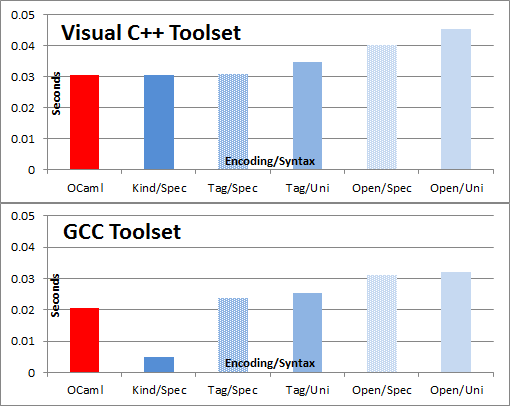
\includegraphics[width=0.47\textwidth]{OCamlComparison.png}
  \caption{Performance comparison of various encodings and syntax against OCaml code}
  \label{fig:OCamlComparison}
\end{figure}

We can see that the use of specialized syntax on a closed/sealed hierarchy can 
match the speed of, and even be four times faster than, the code generated by 
the native OCaml compiler. Once we go for an open solution, we become about 
30-50\% slower. 

\subsection{Qualitative Comparison}
\label{sec:qualcmp}

For this experiment we have reimplemented a visitor based C++ pretty printer for 
Pivot's IPR using our pattern matching library. Most of the rewrite was 
performed by sed-like replaces that converted visit methods into respective 
case-clauses. In several cases we had to manually reorder case-clauses to avoid 
redundancy as visit-methods for base classes were typically coming before the 
same for derived, while for pattern matching we needed them to come after. 
Redundancy checking support in the library discussed in \textsection\ref{sec:redun}
was invaluable in finding out all such cases.

During this refactoring we have made several simplifications that became obvious 
in pattern-matching code, but were not in visitors code because of control 
inversion. Simplifications that were applicable to visitors code were eventually 
integrated into visitors code as well to make sure we do not compare 
algorithmically different code. In any case we were making sure that both 
approaches regardless of simplifications were producing byte-to-byte the same 
output as the original pretty printer we started from.

The size of executable for pattern matching approach was smaller than that for 
visitors. So was also the source code. We extracted from both sources the 
functionality that was common to them and placed it in a separate translation 
unit to make sure it does not participate in the comparison. We kept all the 
comments however that were eqaully applicable to code in either approach.

Note that the visitors involved in the pretty printer above did not use 
forwarding: since all the C++ constructs were handled by the printer, every 
visit-method was overriden from those statically possible based on the static 
type of the argument.

%Listing parameter for a case clause always causes access to member. Best hope is 
%that compiler will eliminate it if it is not needed. At the moment we do not 
%have means to detect empty macro arguments or \_.

%To be continued...

In general from our rewriting experience we will not recommend rewriting 
existing visitor code with pattern matching for the simple reason that pattern 
matching code will likely follow the structure already set by the visitors. 
Pattern matching was most effective when writing new code, where we could design 
the structure of the code having the pattern matching facility in our toolbox.
